\chapter{Implied Volatility, the Vol Surface, and Gamma Scalping}
\label{ch:vol_surface}
\chaptermark{Vol surface and gamma scalping}

Black--Scholes takes volatility as an input, but the market's call
price \emph{already encodes} the volatility the market expects:
given any observed call quote, there is a unique $\volat$ that,
fed through the Black--Scholes formula of \cref{ch:black_scholes},
reproduces the quote exactly. Inverting Black--Scholes to back out
that number is \emph{implied volatility}. It depends on strike, on
maturity, and on the moment you ask --- producing a whole
\emph{surface} of implied vols rather than a single number. This
chapter explains the surface: how it is built, how to read it, why
it is not the flat plane Black--Scholes assumes, and how traders
exploit it. The payoff is \emph{gamma scalping}: buy cheap vol,
delta-hedge against the underlying, and collect the
realised-vs-implied gap from \cref{ch:greeks_hedging}. Gamma
scalping is the canonical vol trade and the reason every
derivatives desk runs a Greeks-based risk book.

Two objectives. First, define implied volatility formally, describe
the inversion procedure, and catalogue the four qualitative
features of the empirical surface (smile, skew,
short-vs-long-dated shape, term structure). Second, turn the P\&L
identity of \cref{ch:greeks_hedging} into a rule: buy options
whose implied vol is below your forecast of realised vol, short
the underlying in the BS-delta amount, rebalance on a schedule,
collect the gap. Variance swaps appear qualitatively here; the
full replication argument is deferred to
\cref{ch:equity_derivatives}.

\begin{backgroundbox}[Prerequisites]
From earlier in the book:
\begin{itemize}
  \item \Cref{ch:black_scholes}: the Black--Scholes European call
  price
  \begin{equation*}
    \Call \;=\; \Spx\,\CDFN(d_1) \;-\; \Kstrike\,e^{-\rrf(\Tmat-t)}\,\CDFN(d_2),
  \end{equation*}
  with $d_1 = [\ln(\Spx/\Kstrike) + (\rrf + \tfrac12 \volat^2)(\Tmat
  - t)]/(\volat\sqrt{\Tmat - t})$ and $d_2 = d_1 - \volat\sqrt{\Tmat
  - t}$, together with the running numerical anchor $\Spx =
  \Kstrike = 100$, $\rrf = 5\%$, $\volat = 20\%$, $\Tmat - t = 1$,
  $d_1 = 0.35$, $d_2 = 0.15$, $\Call \approx 10.4506$.
  \item \Cref{ch:greeks_hedging}: the five primary Greeks, in
  particular $\Delta = \CDFN(d_1)$, $\Gamma =
  \pdfN(d_1)/(\Spx\,\volat\,\sqrt\tau)$, and
  $\nu = \Spx\sqrt\tau\,\pdfN(d_1)$; the Black--Scholes PDE
  $\Theta + \rrf\Spx\,\Delta + \tfrac12\volat^2\Spx^2\,\Gamma =
  \rrf\,\Call$; and the delta-hedged P\&L identity
  \begin{equation*}
    d\Pi \;\approx\; \tfrac12\,\Gamma\,\Spx^2\,
    \bigl(\volat_{\text{r}}^2 - \volat_{\text{i}}^2\bigr)\,dt,
  \end{equation*}
  which this chapter turns into a trading rule.
  \item \Cref{ch:options_payoffs}: put--call parity and the
  no-arbitrage bounds. Parity implies that a call and a put at the
  same $(\Kstrike, \Tmat)$ have the same implied vol, so the
  surface is labelled by $(\Kstrike, \Tmat)$ alone, not by
  call-versus-put.
\end{itemize}
From outside the book:
\begin{itemize}
  \item Root-finding at the level of bisection or Newton--Raphson.
  One-dimensional root finding on a monotone function is all the
  inversion machinery this chapter needs.
  \item Multivariable functions and their level sets --- enough to
  visualise a surface over a $(\Kstrike, \Tmat)$ plane.
\end{itemize}
\end{backgroundbox}

\begin{intuitionbox}
``SPX vol is $18\%$'' is a lie of convenience. The market believes
in a different volatility for every strike and maturity, and the
pattern encodes everything Black--Scholes ignored (fat tails, crash
risk, clustered moves, leverage effects). The surface records
those beliefs in a form still tradable against Black--Scholes.
Reading it tells a derivatives trader in under a minute what the
rest of the market thinks is about to happen.
\end{intuitionbox}

\section{Implied volatility}
\label{sec:ch17_iv}

\begin{definition}[Implied volatility]
\index{implied volatility|textbf}\index{volatility!implied|textbf}
\label{def:implied_vol}
Fix the observable market inputs $(\Spx, \Kstrike, \rrf, \Tmat -
t)$ for a European call, and let $\Call^{\text{mkt}}$ be the call's
observed mid-market price. The \emph{implied volatility} of the
call, written $\volat_{\text{imp}}$, is the unique value of the
volatility parameter $\volat$ that, when substituted into the
Black--Scholes formula
\begin{equation}
  \Call^{\text{BS}}(\Spx,\Kstrike,\rrf,\volat,\Tmat-t)
  \;=\; \Spx\,\CDFN(d_1(\volat)) \;-\; \Kstrike\,e^{-\rrf(\Tmat-t)}\,\CDFN(d_2(\volat)),
  \label{eq:iv_def}
\end{equation}
reproduces the observed price $\Call^{\text{mkt}}$:
\begin{equation}
  \Call^{\text{BS}}(\Spx,\Kstrike,\rrf,\volat_{\text{imp}},\Tmat-t)
  \;=\; \Call^{\text{mkt}}.
  \label{eq:iv_equation}
\end{equation}
\end{definition}

Two remarks. First, the definition applies to puts too: put--call
parity (\cref{ch:options_payoffs}) is model-free, so a call and
put at the same $(\Kstrike, \Tmat)$ must share
$\volat_{\text{imp}}$. Second, existence and uniqueness follow
from monotonicity: vega
$\nu = \Spx\sqrt{\Tmat-t}\,\pdfN(d_1) > 0$
(\cref{ch:greeks_hedging}), so \eqref{eq:iv_def} is strictly
increasing in $\volat$ on $(0, \infty)$, ranging from
$\max(\Spx - \Kstrike e^{-\rrf(\Tmat-t)},\,0)$ at $\volat = 0$ to
$\Spx$ as $\volat \to \infty$. Any price inside those bounds is
hit by exactly one $\volat_{\text{imp}}$.

\subsection{Inverting Black--Scholes numerically}
\label{subsec:ch17_inversion}

No closed form inverts \eqref{eq:iv_def} in $\volat$: the formula
mixes $\volat$ both multiplicatively (in $d_1$) and inside the
normal CDF. But since the call price is strictly monotone and
smooth in $\volat$, one-dimensional root finders converge quickly.
Two choices dominate practice:

\begin{enumerate}
  \item \textbf{Bisection.} Robust but slow. Bracket in
  $[10^{-6},\,5]$ (5 covers every exchange-traded underlying; vol
  has never been quoted above $500\%$) and halve on each step.
  Reaches machine precision in $\sim 50$ iterations.
  \item \textbf{Newton--Raphson.} Uses vega as the derivative:
  $\volat_{n+1} = \volat_n - (\Call^{\text{BS}}(\volat_n) -
  \Call^{\text{mkt}})/\nu(\volat_n)$. Converges quadratically,
  typically in $3$--$5$ iterations. Fails if a step overshoots
  the feasible interval; standard fix is to fall back to bisection.
\end{enumerate}

Production systems use ``safeguarded Newton'', bisecting whenever a
Newton step leaves the bracket. Scipy's \texttt{brentq} is such a
hybrid; \S\ref{sec:ch17_code} uses it.

\begin{keyfactbox}[Implied volatility as a quoting convention]
On every derivatives desk and every options exchange, options are
quoted in \emph{vol}, not dollars. A statement like ``the $25$-delta
$3$-month \texttt{AAPL} put is trading at $32$ vol'' means the
market-observed put premium corresponds to an implied volatility of
$\volat_{\text{imp}} = 32\%$ in the Black--Scholes formula at that
strike and maturity. The dollar premium is computable from
$\volat_{\text{imp}}$, $\Spx$, and $\rrf$ by one call to
$\Call^{\text{BS}}$ or $\Put^{\text{BS}}$.
\end{keyfactbox}

\subsection{Why vol, not dollars}
\label{subsec:ch17_why_vol}

Pricing in vol is pragmatic, not theoretical. Three reasons.

\emph{Stability across strikes.} A $\Kstrike = 90$ and
$\Kstrike = 110$ call have very different dollar prices but
comparable implied vols. Mispricings jump out on a vol ladder
(one strike at $21$ vol when its neighbours are at $18$) that
would be hidden on a dollar ladder by intrinsic-value noise.

\emph{Stability across maturities.} A $1$-month and $1$-year call
have very different premia but comparable implied vols; quoting in
vol factors out the $\sqrt{\Tmat - t}$ scaling every option premium
obeys.

\emph{Stability across spot moves.} If spot rallies $2\%$, every
call's dollar price rallies with it, but implied vols barely move
(the \emph{sticky-delta} convention of \S\ref{sec:ch17_sticky}
makes this almost exact). Vol is roughly conserved under the one
noise dimension that would otherwise swamp any quote.

A derivatives desk's screens therefore show strikes $\times$
maturities with an implied vol in each cell (bid, ask, mid, diff
from yesterday), not dollar prices.

\subsection{A worked inversion}
\label{subsec:ch17_worked_iv}

Take the running anchor from \cref{ch:black_scholes}:
$\Spx = \Kstrike = 100$, $\rrf = 0.05$, $\Tmat - t = 1$. At
$\volat = 0.20$:
\begin{equation*}
  \Call^{\text{BS}}(100, 100, 0.05, 0.20, 1) \;\approx\; 10.4506.
\end{equation*}
Suppose the market shows a richer price,
$\Call^{\text{mkt}} = 11.50$. Since vega is positive, the implied
vol must exceed $0.20$. Bracketing in $[0.10, 0.40]$:
$\Call^{\text{BS}}(\ldots,0.10,1) \approx 6.80 < 11.50$ and
$\Call^{\text{BS}}(\ldots,0.40,1) \approx 18.02 > 11.50$, so the
root is inside. Brent to machine precision yields
\begin{equation*}
  \volat_{\text{imp}} \;\approx\; 0.22788 \;=\; 22.79\%.
\end{equation*}
The ATM year call is priced at $22.79$ vol, a $2.79$-point premium
over the ``true'' $20$ vol. A trader forecasting realised at
$20\%$ reads this as a sell signal: delta-hedged short harvests,
by the P\&L identity of \cref{ch:greeks_hedging}, roughly
$\tfrac12 \Gamma \Spx^2 (\volat_{\text{imp}}^2 -
\volat_{\text{real}}^2) \approx 93.81 \cdot (0.22788^2 - 0.20^2)
\approx \$1.12$ per year of gamma exposure. Seed of gamma
scalping; developed in \S\ref{sec:ch17_gamma_scalping}.

Round-trip sanity: feed $\volat = 0.20$ through BS and invert
$\Call = 10.4506$ back; Brent returns $0.20000$ to six decimals.
Any production IV inverter should satisfy
$\text{IV}(\text{BS}(\volat)) = \volat$ to within $10^{-6}$ over
the full $(\volat, \Kstrike, \Tmat)$ grid.

\section{The vol surface}
\label{sec:ch17_surface}

Now vary $\Kstrike$ and $\Tmat$. Each liquid option is a point
$(\Kstrike_i, \Tmat_j)$ with a market price
$\Call^{\text{mkt}}_{i,j}$ and an implied vol
$\volat_{\text{imp}}(\Kstrike_i, \Tmat_j)$ from the inversion of
\S\ref{subsec:ch17_inversion}. Plotting them gives a surface:

\begin{definition}[Vol surface]
\index{volatility surface|textbf}\index{volatility!surface|textbf}
\label{def:vol_surface}
Fix an underlying and an instant in time. The \emph{vol surface}
(also called \emph{implied vol surface} or simply \emph{surface})
is the function
\begin{equation*}
  (\Kstrike, \Tmat) \;\mapsto\; \volat_{\text{imp}}(\Kstrike, \Tmat),
\end{equation*}
defined on the strike--maturity plane wherever a liquid option
quote exists. Intermediate points are interpolated (bilinearly for
simple desks, via a parametric model --- SABR or SVI --- on
production desks). The interpolation matters because most desks
quote exotics and bespoke OTC options at strikes and expiries
that do not trade on exchange: reading $\volat_{\text{imp}}$ off
the calibrated surface and feeding it through BS is how those
off-grid options get priced.
\end{definition}

If Black--Scholes were the truth, the surface would be flat:
$\volat_{\text{imp}}(\Kstrike, \Tmat) \equiv \volat$. It is not.
The true return distribution has fatter tails than the lognormal
BS assumes, so wherever the market assigns more probability than
BS does --- far-OTM strikes, near-term expiries across a known
event --- options there are worth more than BS says, and the only
way to reconcile the richer market price with the BS formula is
to feed in a higher $\volat$.
\Citeauthor{bennett2014trading} \citeBennett Ch 4, \citeNatenberg\
Ch 13, and \citeHull\ Ch 18 all show that the surface has systematic
structure on both axes, stable enough that practitioners trade the
shape itself.

\subsection{Cross-sections: smile, skew, term structure}
\label{subsec:ch17_cross_sections}

The surface is easier to read as two one-dimensional cross-sections
than as a 2D plot.

\paragraph{Strike cross-section (smile / skew).}
Fix $\Tmat$ and plot $\volat_{\text{imp}}$ against $\Kstrike$ (or
moneyness $m = \ln(\Kstrike/\Spx)$, or BS delta). \emph{Smile}
when roughly symmetric and U-shaped; \emph{skew} when it slopes
in one direction.

\begin{definition}[Smile and skew]
\index{volatility smile|textbf}\index{volatility skew|textbf}
\label{def:smile_skew}
The \emph{volatility smile} is a strike cross-section of the vol
surface whose implied vol is higher at out-of-the-money strikes
(both tails, put and call) than at the at-the-money strike, giving
the curve a U or smile shape. The \emph{volatility skew} is the
asymmetric version: for most equity underlyings the left wing
(low strikes, far OTM puts and far ITM calls) rises faster than
the right wing, giving a downward-sloping curve.
\end{definition}

Equity indices skew because crashes are one-sided: investors fear
downside gaps but not upside ones, so OTM puts are bid above OTM
calls. FX pairs smile because either currency can collapse
relative to the other, so both tails get bid equally.

\begin{figure}[ht]
\centering
\begin{minipage}{0.48\textwidth}
\centering
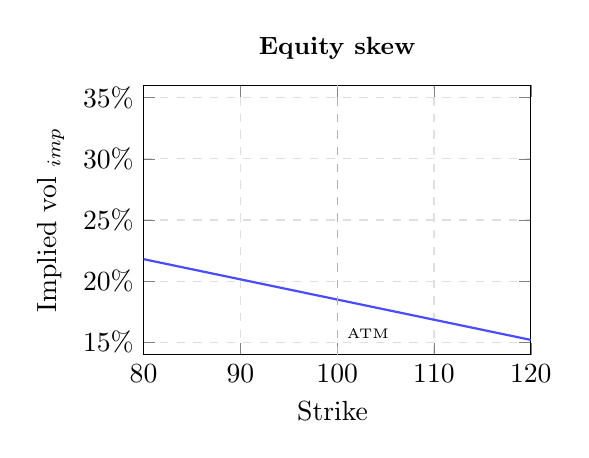
\begin{tikzpicture}
\begin{axis}[
  width=6.5cm, height=5cm,
  xlabel={Strike $\Kstrike$},
  ylabel={Implied vol $\volat_{\text{imp}}$},
  xmin=80, xmax=120,
  ymin=0.14, ymax=0.36,
  xtick={80,90,100,110,120},
  ytick={0.15,0.20,0.25,0.30,0.35},
  yticklabels={15\%,20\%,25\%,30\%,35\%},
  title={Equity skew},
  title style={font=\small\bfseries},
  grid=major, grid style={dashed,gray!25},
]
\addplot[blue!70, thick, domain=80:120, samples=40]
  {0.185 + 0.00165*(100-x)};
\addplot[dashed, gray!60, thin] coordinates {(100,0.14)(100,0.36)};
\node[font=\tiny, above right] at (axis cs:100,0.145) {ATM};
\end{axis}
\end{tikzpicture}
\end{minipage}
\hfill
\begin{minipage}{0.48\textwidth}
\centering
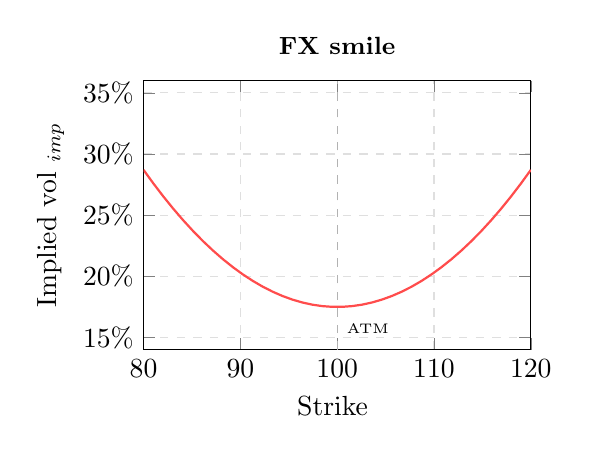
\begin{tikzpicture}
\begin{axis}[
  width=6.5cm, height=5cm,
  xlabel={Strike $\Kstrike$},
  ylabel={Implied vol $\volat_{\text{imp}}$},
  xmin=80, xmax=120,
  ymin=0.14, ymax=0.36,
  xtick={80,90,100,110,120},
  ytick={0.15,0.20,0.25,0.30,0.35},
  yticklabels={15\%,20\%,25\%,30\%,35\%},
  title={FX smile},
  title style={font=\small\bfseries},
  grid=major, grid style={dashed,gray!25},
]
\addplot[red!70, thick, domain=80:120, samples=40]
  {0.175 + 0.00028*(x-100)^2};
\addplot[dashed, gray!60, thin] coordinates {(100,0.14)(100,0.36)};
\node[font=\tiny, above right] at (axis cs:100,0.145) {ATM};
\end{axis}
\end{tikzpicture}
\end{minipage}
\caption{Two common vol-surface shapes in practice. \textbf{Equity skew} (left):
implied vol falls as strike rises. OTM puts are expensive because investors
pay a premium for crash protection, so the left wing of the smile is elevated.
\textbf{FX smile} (right): implied vol is roughly symmetric and U-shaped,
reflecting comparable demand for OTM calls and puts.
Both shapes contradict Black--Scholes's assumption of a flat, constant vol.}
\label{fig:vol_skew_smile}
\end{figure}

\paragraph{Maturity cross-section (term structure).}
Fix $\Kstrike$ and plot $\volat_{\text{imp}}(\Kstrike,\Tmat)$
against $\Tmat$ to get the \emph{volatility term structure}.
Calm markets: upward-sloping (\emph{contango}; more uncertainty
over a year than a month). Stressed markets: inverted
(\emph{backwardation}; a near-term event is being priced in).

\subsection{Four canonical shapes to memorise}
\label{subsec:ch17_four_shapes}

\citeBennett, \citeNatenberg, and \citeHull\ converge on four
qualitative observations. They are the phrasebook you need on an
options desk.

\paragraph{(1) Short-dated strike cross-section: sharp smile.}
A one- or two-week expiry against moneyness shows a sharp U: ATM
is a well, both wings rise steeply. A $10$-delta OTM put at one
week might trade at $45$ vol vs ATM at $20$ --- a $25$-point
premium. Tail risk over the next week is disproportionately
priced; short-dated crash insurance is expensive.

\paragraph{(2) Long-dated strike cross-section: flatter shape.}
A one-year expiry on the same underlying shows a gentler curve;
wings rise by perhaps $3$--$5$ points rather than $25$. Over
longer horizons the return distribution is closer to Gaussian
(CLT), and Black--Scholes fits the tail better.

\paragraph{(3) Equity-index skew: downward slope.}
SPX, SX5E, N225, and other major indices exhibit a persistent
downward skew: the strike cross-section slopes down from low to
high strikes. A $90$-strike SPX put at three months might imply
$25$ vol, ATM $18$, $110$-strike call $16$. Demand for downside
crash protection structurally exceeds demand for upside
speculation, so put implied vol is bid above call implied vol
(more in \S\ref{subsec:ch17_smile_origin}).

\paragraph{(4) ATM term structure: contango vs backwardation.}
Normal markets: ATM vol slopes up with maturity
($1$-month $<$ $3$-month $<$ $6$-month $<$ $1$-year). Typical SPX
calm: $14, 16, 17, 18$ vol. Stress (Brexit 2016, COVID 2020,
GFC 2008): inverted, $1$-month spikes to $40$ while $1$-year only
moves to $25$.

\begin{keyfactbox}[The vol surface]
The \emph{vol surface} is the function $(\Kstrike, \Tmat) \mapsto
\volat_{\text{imp}}(\Kstrike, \Tmat)$ obtained by inverting
Black--Scholes against every liquid option quote on a given
underlying at a given instant. Empirically the surface is never
flat. It exhibits (a) a \emph{smile} or \emph{skew} along the
strike axis, sharper at short maturities and flatter at long
maturities, with a persistent downward skew on equity indices;
and (b) a \emph{term structure} along the maturity axis, typically
upward-sloping (contango) in calm markets and downward-sloping
(backwardation) in stress. Reading the surface is how a
derivatives trader diagnoses what the market is pricing in.
\end{keyfactbox}

\begin{intuitionbox}
The vol surface is the market's \emph{correction} to Black--Scholes.
BS assumes constant vol; the surface records that it isn't. A
derivatives desk never uses BS with a single vol: it uses BS plus
a \emph{calibrated surface}, so every option it prices is
consistent with every other option in the market. The formula is
a local coordinate; the surface is the global manifold; traders
trade positions in that manifold.
\end{intuitionbox}

\subsection{Where the smile came from: the 1987 crash}
\label{subsec:ch17_smile_origin}

Before October 1987, listed option quotes across strikes traded
at roughly the same implied vol --- the smile did not exist. Flat
vol was a pillar of early BS empirical validation.

\begin{historybox}
On \textbf{Monday, October 19, 1987} --- Black Monday --- the
S\&P $500$ fell $20.5\%$ in one session. Under BS with the
$15$--$18$ vol equity options were trading at, the implied
probability of a $-20\%$ daily move was roughly $10^{-59}$. Reality
disagreed.

From Tuesday onward, traders re-priced far-OTM puts to much
higher vols than ATM: the crash had shown the tail was far fatter
than BS assumed, and crash insurance became permanently bid.
\Citeauthor{derman2004mylife} \citeDerman\ Ch 9 describes the
floor's overnight reshaping; the constant-vol framework was
replaced by the vol-surface framework within two weeks. The smile
has never gone away. \Citeauthor{bennett2014trading}
\citeBennett\ is the canonical practitioner reference; free to
download and required reading for this chapter.
\end{historybox}

\section{Sticky strike vs sticky delta}
\label{sec:ch17_sticky}

The surface depends on the current spot $\Spx$ through a strike's
relationship to ATM. When spot moves, the surface moves with it;
two competing conventions describe \emph{how}.

\begin{definition}[Sticky strike]
\index{sticky strike|textbf}
Under the \emph{sticky-strike} assumption, the implied volatility
at a fixed strike $\Kstrike$ is invariant to the underlying's
level: if SPX moves from $\Spx = 4000$ to $\Spx = 4050$, the
implied vol of the $\Kstrike = 4000$ call stays the same. The
entire smile remains pinned to absolute strike levels.
\end{definition}

\begin{definition}[Sticky delta]
\index{sticky delta|textbf}
Under the \emph{sticky-delta} assumption (sometimes called
\emph{sticky moneyness}), the implied volatility at a fixed
Black--Scholes delta --- equivalently, at a fixed moneyness $m
= \ln(\Kstrike/\Spx)$ --- is invariant to the underlying's level.
If SPX moves from $4000$ to $4050$, the entire smile
\emph{translates} with the spot: the $25$-delta put vol stays
where it was, but the strike that gives $25$ delta has moved.
\end{definition}

These differ in how the surface moves with $\Spx$, and hence in
the correct delta hedge.

\subsection{Effect on model delta}
\label{subsec:ch17_sticky_delta}

BS delta $\CDFN(d_1)$ was derived with $\volat$ independent of
$\Spx$. Under sticky-delta, moving $\Spx$ also moves the implied
vol of the strike I hold (its moneyness changed), so the
``effective'' delta picks up an extra term. Write the call price
as a function of $\Spx$ through both channels:
\begin{equation*}
  \Call(\Spx) \;=\; \Call^{\text{BS}}\bigl(\Spx, \Kstrike, \rrf,\,
                   \volat_{\text{imp}}(\Spx),\,\Tmat - t\bigr),
\end{equation*}
where under sticky-delta $\volat_{\text{imp}}(\Spx)$ is the
implied vol of the point on the surface that has moved with the
spot. Applying the chain rule,
\begin{equation}
  \frac{d\Call}{d\Spx} \;=\;
    \underbrace{\frac{\partial \Call^{\text{BS}}}{\partial \Spx}}_{\text{BS delta}}
    \;+\; \underbrace{\frac{\partial \Call^{\text{BS}}}{\partial \volat}}_{\text{vega}}
          \cdot
          \underbrace{\frac{d\volat_{\text{imp}}}{d\Spx}}_{\text{``skew slide''}}.
  \label{eq:sticky_delta_effective}
\end{equation}
The first term is the usual $\CDFN(d_1)$; the second corrects for
how implied vol moves with spot. On an equity index with a downward
skew and sticky-delta dynamics, $d\volat_{\text{imp}}/d\Spx < 0$
(a rally slides my strike rightward along the downward skew, so
its implied vol drops); vega is positive, so the correction
\emph{reduces} effective delta below BS. A fall does the reverse.

Sticky-strike is the limit $d\volat_{\text{imp}}/d\Spx = 0$:
effective delta equals BS delta.

\begin{keyfactbox}[Sticky-strike vs sticky-delta effective delta]
\begin{align*}
  \Delta_{\text{effective}}^{\text{sticky strike}} \;&=\; \Delta^{\text{BS}}, \\
  \Delta_{\text{effective}}^{\text{sticky delta}}  \;&=\; \Delta^{\text{BS}}
        \;+\; \nu \cdot \frac{d\volat_{\text{imp}}}{d\Spx}.
\end{align*}
The correction term is negative for equity indices (downward
skew implies $d\volat_{\text{imp}}/d\Spx < 0$), so sticky-delta
hedging on an equity book uses a \emph{smaller} share count than
BS delta would suggest.
\end{keyfactbox}

\subsection{Which convention is empirically right?}
\label{subsec:ch17_convention_choice}

Both conventions are stylised; neither is exactly right.
\Citeauthor{bennett2014trading} \citeBennett\ Ch 5 gives the
empirical breakdown: equity indices tend to sticky-delta in calm
regimes (smile translates with spot) and sticky-strike in stress
(smile steepens). Single names are more sticky-strike; FX is
sticky-delta; rates have their own conventions
(sticky-log-normal, or sticky-basis-point OTC).

Desks pick one convention, backtest it against recent spot moves,
and adjust the model delta accordingly.

\begin{pitfallbox}[The ``BS delta'' depends on your sticky convention]
Using raw $\CDFN(d_1)$ as a hedge ratio on an equity-index option
implicitly assumes sticky-strike. If the market is sticky-delta
(usual for SPX in calm regimes), the hedge is wrong and the
``hedged'' P\&L drifts systematically with spot. Every desk
corrects the model delta for its chosen convention:
$\Delta^{\text{BS}} + \nu \cdot d\volat_{\text{imp}}/d\Spx$, with
the slide estimated from the observed skew. Ignoring this costs a
long-dated equity market-making book several basis points a day
in unexplained P\&L.
\end{pitfallbox}

\section{Variance swaps (qualitative)}
\label{sec:ch17_varswap}

The vol surface is read by eye and traded one option at a time,
but a second product trades \emph{pure} volatility directly: the
\emph{variance swap}. Full replication is deferred to
\cref{ch:equity_derivatives}; here we give the intuition, a
schematic formula, and why variance swaps are the cleanest vol
trade on a sell-side desk.

\begin{definition}[Variance swap]
\index{variance swap|textbf}
\label{def:varswap}
A \emph{variance swap} on an underlying $\Spx$ is an OTC derivative
with the following cashflow at maturity $\Tmat$:
\begin{equation*}
  \text{Payoff} \;=\; N \,\cdot\, \bigl(\,\volat_{\text{realised}}^2(0,\Tmat)
                      \;-\; \Kstrike_{\text{var}}^2\,\bigr),
\end{equation*}
where $\volat_{\text{realised}}^2(0,\Tmat)$ is the realised
variance of $\ln(\Spx)$ over $[0,\Tmat]$, $\Kstrike_{\text{var}}$
is the \emph{variance strike} (expressed in vol units and squared
at settlement), and $N$ is a notional chosen so that a
$1$-vol-point move in realised vol corresponds to a fixed dollar
P\&L (the ``vega notional'' convention). The swap pays nothing at
initiation; $\Kstrike_{\text{var}}$ is set at trade time so that
the expected risk-neutral value of the payoff is zero.
\end{definition}

A variance swap is a pure bet on realised volatility. Unlike a
delta-hedged option (with residual path-dependence,
gamma-non-uniformity, and discrete-hedging risks of
\cref{ch:greeks_hedging}), its payoff is the integral of squared
returns alone: no gamma to manage, no rebalancing schedule, no
path where realised is ``high'' but the position loses from bad
hedge timing. If realised variance exceeds the strike, you win
by the excess.

\subsection{Replication via a strip of OTM options}
\label{subsec:ch17_varswap_replication}

Demeterfi--Derman--Kamal--Zou showed (expanded in \citeBennett\
Ch 12 and \citeHull\ Ch 26) that a variance swap is replicable
\emph{model-independently} by a static European-option portfolio
plus a dynamic forward position. The option leg is a continuous
strip of OTM puts and calls, weighted by $1/\Kstrike^2$:

\begin{keyfactbox}[Variance swap replication (schematic)]
A $T$-maturity variance swap on a non-dividend-paying underlying
with forward $F_0 = \Spx_0 e^{\rrf T}$ is replicated by holding,
at time $0$:
\begin{multline}
  \Pi^{\text{static}}
  \;=\; \frac{2}{T}\left[\;
          \int_0^{F_0}\frac{\Put(\Kstrike)}{\Kstrike^2}\,d\Kstrike
          \;+\;
          \int_{F_0}^{\infty}\frac{\Call(\Kstrike)}{\Kstrike^2}\,d\Kstrike
        \right] \\
  \;-\; \text{(dynamic forward hedge)},
  \label{eq:varswap_replication}
\end{multline}
where the continuous integrals are understood as a sum over
available strikes with weights $w_i \propto 1/\Kstrike_i^2$. At
maturity this static portfolio pays exactly the realised variance
$\volat_{\text{realised}}^2(0,\Tmat)$, up to a residual that
vanishes as the strike grid becomes finer.
\end{keyfactbox}

The derivation --- the log-payoff $2\ln(F_T/F_0)$ is replicable as
a $1/\Kstrike^2$-weighted integral over OTM puts and calls --- is
in \cref{ch:equity_derivatives} and \citeHull\ \S26.16. Three
structural takeaways:

\emph{The $1/\Kstrike^2$ weight is not a fudge.} It matches the
second derivative of the log-payoff w.r.t.\ the forward. Any other
weighting replicates a different payoff.

\emph{Variance swaps are long convexity.} Variance is vol squared,
so a doubling of vol quadruples the payoff. A \emph{volatility
swap} (linear in $\volat_{\text{realised}}$) lacks this convexity,
is harder to replicate, and is usually priced as a variance swap
plus a convexity correction.

\emph{OTM puts get the lion's share.} Low strikes contribute
disproportionately under $1/\Kstrike^2$; SPX variance swaps are
dominated by OTM put exposure, so their bid/offer tracks put skew
closely.

\begin{intuitionbox}
A variance swap is what a delta-hedged option aspires to be
--- a pure vol bet --- but without the gamma-path and
discrete-hedging noise. The replication formula says: stop hedging
one call; hold a weighted strip of every OTM option, and the
strip itself prices pure variance. Sell-side desks quote the
strip and trade it against OTC variance-swap confirms.
Variance-swap trading is \emph{industrial-scale} gamma scalping.
\end{intuitionbox}

\Cref{ch:equity_derivatives} gives the full DDKZ derivation, the
variance-vs-volatility-swap convexity correction, and the desk
workflow for a typical variance-swap ticket.

\section{Gamma scalping as an explicit strategy}
\label{sec:ch17_gamma_scalping}

We turn the P\&L identity of \cref{ch:greeks_hedging} into a
rule. For a delta-hedged long-option position,
\begin{equation}
  d\Pi \;\approx\; \tfrac12\,\Gamma\,\Spx^2\,
                   \bigl(\,\volat_{\text{r}}^2 \;-\; \volat_{\text{i}}^2\,\bigr)\,dt.
  \label{eq:ch17_vol_trading_eq}
\end{equation}
Every P\&L dollar on a delta-hedged book is the integrated
realised-minus-implied gap weighted by gamma. The market prices
$\volat_{\text{i}}$ through the surface; a trader who believes
realised will exceed implied has a directly actionable rule: buy
the option, delta-hedge, collect the gap. That is gamma scalping.

\subsection{The strategy rule}
\label{subsec:ch17_gs_rule}

\begin{definition}[Gamma scalping]
\index{gamma scalping|textbf}
\label{def:gamma_scalping}
\emph{Gamma scalping} is the strategy of (i) buying an option (or
a basket of options) whose implied volatility is below the
trader's forecast of realised volatility over the option's life;
(ii) simultaneously shorting the underlying in the Black--Scholes
delta amount to remain approximately delta-neutral; (iii)
rebalancing the delta hedge on a fixed schedule (every $K$ ticks,
every $\$\delta$ of spot move, or every $T/N$ seconds); and (iv)
collecting the cumulative
$\tfrac12 \Gamma (\Delta\Spx)^2$ slugs against the theta cost of
holding the option.
\end{definition}

Step by step, running against the chapter's running example
($\Spx_0 = 100$, $\Kstrike = 100$, $\rrf = 5\%$, $\Tmat = 1$,
implied $\volat_{\text{i}} = 20\%$):

\begin{enumerate}
  \item \textbf{Forecast realised vol.} From trailing $30$-day
  realised vol of log-returns, or a GARCH/ARMA forecast, project
  $\volat_{\text{r}}$. Suppose $\volat_{\text{r}} = 25\%$, $5$
  points above implied.
  \item \textbf{Price-check each strike.} Invert every liquid
  quote to $\volat_{\text{imp}}(\Kstrike_i)$. Any strike with
  $\volat_{\text{imp}} < \volat_{\text{r}}$ is a buy candidate.
  Here the ATM call at $20$ vs a forecast of $25$ qualifies.
  \item \textbf{Buy the option.} Pay $\Call \approx 10.4506$ per
  unit; record entry $\volat_{\text{imp}} = 0.20$.
  \item \textbf{Short the delta.} $\Delta \approx 0.6368$, so
  short $0.6368$ shares per call to go delta-neutral.
  \item \textbf{Rebalance on a schedule.} As $\Spx$ drifts, the
  call's delta drifts too; reset the share hedge each rebalance.
  \item \textbf{Cumulative P\&L.} Each window books
  $\tfrac12 \Gamma (\Delta\Spx)^2 - \text{theta}$; over the year
  the integral approaches
  $\tfrac12 \Gamma \Spx^2 (\volat_{\text{r}}^2 -
  \volat_{\text{i}}^2) \Tmat$.
  \item \textbf{Exit.} Either close out before expiry (booking the
  cumulative gamma P\&L) or hold to expiry (call payoff plus
  cumulative hedge P\&L gives the same total).
\end{enumerate}

\subsection{The numerical example}
\label{subsec:ch17_gs_numbers}

At the anchor, $\tfrac12 \Gamma \Spx^2 = \tfrac12 \cdot 0.01876
\cdot 100^2 = 93.81$ dollars per $\text{vol}^2$-year. If realised
prints at $25\%$ against implied $20\%$:
\begin{align*}
  \tfrac12\,\Gamma\,\Spx^2\,(\volat_{\text{r}}^2 - \volat_{\text{i}}^2)
  \;&=\; 93.81 \cdot (0.0625 - 0.04) \\
  \;&=\; 93.81 \cdot 0.0225 \\
  \;&\approx\; \$2.11 \text{ per unit of call, per year}.
\end{align*}
Against a $\$10.45$ premium, that is $\sim 20\%$ of premium over
one year --- a leveraged, convex, pure play on whether realised
beats $20\%$. Canonical trade of the vol desk.

If the forecast is wrong and $\volat_{\text{r}} = 18\%$, P\&L
flips:
\begin{equation*}
  93.81 \cdot (0.0324 - 0.04) \;=\; -\$0.71 \text{ per unit per year},
\end{equation*}
about $7\%$ of premium bled. Theta dominated the gamma gain. The
failure mode: \emph{you paid for vol and the market didn't
deliver}.

\begin{keyfactbox}[Gamma scalping in one paragraph]
Buy options whose implied vol is below your forecast of realised
vol. Short the Black--Scholes delta in the underlying to stay
neutral. Rebalance the delta on a schedule. Over the life of the
hedge, collect $\sim \tfrac12 \Gamma \Spx^2
(\volat_{\text{r}}^2 - \volat_{\text{i}}^2) \Tmat$ per unit of
call. Win if realised exceeds implied; lose if not. The strategy
\emph{is} the delta-hedged P\&L identity, executed.
\end{keyfactbox}

\begin{intuitionbox}
Gamma scalping trades your vol forecast against the market's
implied. Owning the option is ``long vol''; shorting it is ``short
vol''; delta-hedging strips out direction; what remains is the
pure vol bet. You are not betting on up-or-down --- the hedge
eliminates that --- but on whether the underlying \emph{moves a
lot or a little}. Long gamma profits on every kind of move; you
just need enough, fast enough, to outpace the theta clock.
\end{intuitionbox}

\subsection{Failure modes and subtleties}
\label{subsec:ch17_gs_failures}

Three failure modes bite.

\emph{Realised vol disappoints.} Forecast was $25$, realisation
was $18$, $7\%$ of premium bled. No hedging expertise saves a
wrong vol forecast.

\emph{Implied vol moves during the trade.} The clean
``$\volat_{\text{r}}^2 - \volat_{\text{i}}^2$'' story treats
implied as frozen at entry. In reality the surface fluctuates; an
overnight selloff delivers a vega hit
$\nu \cdot \Delta \volat_{\text{i}}$ unrelated to realised vol. At
the anchor $\nu \approx 37.52$, so a $1$-point drop is $-\$0.375$
on a $\$10.45$ call, $\sim 3.6\%$ of premium. The realised-vs-%
implied story holds only if you exit at the entry
$\volat_{\text{i}}$, or budget for the vega.

\emph{Discrete-hedging error.} \Cref{ch:greeks_hedging} showed
discrete rebalancing adds per-period noise
$\sim \Gamma \Spx^2 \volat^2 \Delta t$. Weekly vs daily gives
$\sim 5\times$ more noise per rebalance but $\sim 5\times$ fewer
rebalances, so cumulative sigma is roughly unchanged; transaction
costs decide. Rebalance frequency is a free parameter; optimising
it is standard work.

\begin{pitfallbox}[Gamma scalping is a vega bet in disguise]
The sloppy pitch --- ``buy the call, delta-hedge, win iff realised
exceeds implied'' --- is not quite right. If implied \emph{rises}
after entry, the long call rallies via vega and you profit
mark-to-market even if realised is average; if implied
\emph{falls}, you lose on vega even if realised is high. The pure
realised-vs-implied story holds only to expiry or if you exit at
entry implied. In practice gamma scalping is partly a vega bet,
and a disciplined desk books realised-vol P\&L and vega P\&L
separately so the trader knows which contributed.
\end{pitfallbox}

\subsection{Regime detection and forward reference}
\label{subsec:ch17_regime}

Whether gamma scalping is right \emph{now} is a regime-detection
question. Calm markets with implied above long-run realised favour
short gamma (vol selling); building macro stress with implied
lagging favours long gamma. The regime-to-strategy decision tree
is in \cref{ch:which_strategy_when}. For now: gamma scalping is
the options-specific wing of a general ``vol forecast vs vol
implied'' framework.

\begin{prosperitybox}
IMC Prosperity 3 introduced \texttt{VOLCANIC\_ROCK\_VOUCHERS} in
Round 3 and kept them through Round 4: five strikes
($9500, 9750, 10000, 10250, 10500$) on \texttt{VOLCANIC\_ROCK}
trading around $10000$, European calls, a few days to expiry.
Inverting each voucher's mid through BS ($\rrf = 0$ in Prosperity)
gives five implied vols at one maturity --- a genuine smile
cross-section.

The top teams' workflow, from the Frankfurt Hedgehogs' second-place
writeup (\cref{ch:top_team_lessons}):
\begin{enumerate}
  \item Invert each voucher's mid to $\volat_{\text{imp}}(\Kstrike)$.
  \item Fit a parabola to get a smooth smile.
  \item Compute residuals $\volat_{\text{imp}} -
  \hat\volat_{\text{smile}}$: negatives are cheap, positives are
  rich.
  \item Buy cheap strikes, sell rich, delta-hedge each with
  \texttt{VOLCANIC\_ROCK} at the BS delta.
\end{enumerate}
Rebalancing every $10$ ticks --- exactly the discrete-hedging
setup above. The ATM $10{,}000$ voucher was the single biggest
P\&L contributor: its implied oscillated around the smile fit,
each oscillation a miniature gamma-scalping round. The Hedgehogs
call IV scalping on \texttt{VOLCANIC\_ROCK\_VOUCHERS} ``a
significant profit centre'' in Rounds 3--4. See
\texttt{imc-prosperity-3/README.md} Rounds 3--4.
\end{prosperitybox}

\begin{gsbox}
A GS equity-derivatives vol-trading Strat's morning ritual is to
\emph{recalibrate the vol surface} to overnight quotes:
\begin{enumerate}
  \item Pull overnight trades and quotes on the coverage universe
  (SPX, SX5E, NDX, RUT, top $200$ US single names).
  \item For each $(\Kstrike, \Tmat)$ with a fresh mid, invert BS
  to $\volat_{\text{imp}}$ via a \texttt{brentq}-style routine
  (\S\ref{sec:ch17_code}). GS's library \texttt{SecDB} holds one
  of the most-called IV inverters on the firm.
  \item Fit a parametric surface. Dominant choices:
  \textbf{SABR} (four-parameter stochastic-vol, smile per
  maturity, closed-form IV approximation) and \textbf{SVI}
  (five-parameter static parameterisation of
  $\volat_{\text{imp}}^2$ in moneyness). Full derivations in
  \cref{ch:equity_derivatives}; here treat as black-box fitters.
  \item Diff against yesterday's surface. Any
  $(\Kstrike, \Tmat)$ moved beyond a threshold
  ($0.5$--$1.0$ points) is flagged.
  \item Trader fades obvious dislocations; risk re-prices the
  book against the calibrated surface, producing fresh P\&L
  attribution and Greeks.
\end{enumerate}
The whole equity-derivatives business --- market making, flow,
exotics, variance swaps, delta-one --- rests on one consistent
calibrated surface. Two desks using different models book
inconsistent P\&Ls and the internal auditors flag within a week.
The surface is a shared operational artefact every risk number
depends on. \Cref{ch:risk_production} returns to the production
engineering.
\end{gsbox}

\section{A short reference implementation}
\label{sec:ch17_code}

The core of every vol-surface pipeline is the IV inverter: a
function taking a market price and returning the BS implied vol.
Minimal version below, using scipy's \texttt{brentq} (safeguarded
Brent; never leaves the bracket). Commit it to muscle memory;
everything else in this chapter calls it.

\begin{lstlisting}[caption={Implied-vol inverter for a European call under Black--Scholes. \texttt{bs\_call} returns the BS price; \texttt{implied\_vol} finds the volatility that reproduces an observed market price via Brent's method. Calling \texttt{implied\_vol(100, 100, 0.05, 1, 10.4506)} returns approximately $0.2000$; calling it on a market price of $11.50$ returns approximately $0.2279$.}]
from scipy.optimize import brentq
from scipy.stats import norm
import math

def bs_call(S, K, r, sigma, T):
    d1 = (math.log(S / K) + (r + sigma ** 2 / 2) * T) / (sigma * math.sqrt(T))
    d2 = d1 - sigma * math.sqrt(T)
    return S * norm.cdf(d1) - K * math.exp(-r * T) * norm.cdf(d2)

def implied_vol(S, K, r, T, C_market):
    f = lambda sigma: bs_call(S, K, r, sigma, T) - C_market
    return brentq(f, 1e-6, 5.0)
\end{lstlisting}

\noindent Two notes. \texttt{brentq} requires a sign-change
bracket; $[10^{-6}, 5]$ covers every realistic equity IV (widen
for exotics above $500\%$). No caching: production adds a Newton
step for speed (Brent $\sim 20$ evals, Newton $\sim 5$) and
caches $d_1, d_2, \CDFN(d_1)$ across Greeks of the same
$(\Spx,\Kstrike,\rrf,\volat,\Tmat)$. The minimal version suffices
for this chapter and any Prosperity workload.

\section{Key facts to memorise}
\label{sec:ch17_key_facts}

\begin{itemize}
  \item \textbf{Implied volatility} of an observed call price
  $\Call^{\text{mkt}}$ is the unique $\volat$ that reproduces
  $\Call^{\text{mkt}}$ when plugged into the Black--Scholes
  formula. Existence and uniqueness follow from the monotonicity
  of the BS price in $\volat$ (vega $> 0$). Inversion is numerical
  --- Brent or Newton --- because there is no closed form.
  \item \textbf{Quoting convention.} Options are quoted in vol
  units, not dollars. A ``$32$-vol'' put means the BS
  inversion of the market premium gives $\volat_{\text{imp}} =
  0.32$. Traders read entire option chains as vol ladders.
  \item \textbf{Round-trip sanity check.} For any vol $\volat$,
  $\text{IV}(\text{BS}(\volat)) = \volat$ to machine precision.
  At the running anchor, $\text{BS}(100, 100, 0.05, 0.20, 1)
  \approx 10.4506$ and $\text{IV}(100, 100, 0.05, 1, 10.4506) =
  0.20000$. This round-trip is the arithmetic-hygiene test of any
  IV pipeline.
  \item \textbf{Vol surface.} The function $(\Kstrike, \Tmat)
  \mapsto \volat_{\text{imp}}(\Kstrike, \Tmat)$. Empirically
  never flat, despite Black--Scholes assuming it should be.
  \item \textbf{Strike cross-section.} Short-dated maturities
  show a sharp U-shaped \emph{smile}; long-dated maturities show
  a flatter curve. On equity indices, the cross-section has a
  persistent downward \emph{skew}: OTM puts trade at higher vol
  than ATM, which trades at higher vol than OTM calls.
  \item \textbf{Maturity cross-section.} \emph{Term structure} of
  ATM vol is upward-sloping (contango) in calm markets and
  inverted (backwardation) in stress. SPX $1$-month vs $1$-year
  ATM in calm: $14$ vs $18$. In March $2020$: $80$ vs $35$.
  \item \textbf{Sticky strike vs sticky delta} distinguishes how
  the surface moves with spot. Sticky strike: vol at absolute
  strike pinned; model delta = BS delta. Sticky delta: vol at
  fixed moneyness pinned, smile translates with spot; model
  delta = BS delta $+ \nu \cdot d\volat_{\text{imp}}/d\Spx$.
  Most equity indices are closer to sticky-delta in calm
  regimes.
  \item \textbf{1987 origin of the smile.} Before Black Monday
  (October 19, 1987), option vols across strikes were roughly
  flat. After the $20.5\%$ single-session crash, OTM puts
  re-priced to pay a permanent crash-insurance premium, and the
  downward equity skew has been in place ever since.
  \item \textbf{Variance swap.} An OTC contract paying
  $\volat_{\text{realised}}^2 - \Kstrike_{\text{var}}^2$ at
  maturity. Replicable by a static $1/\Kstrike^2$-weighted strip
  of OTM puts and calls plus a dynamic forward hedge. The
  cleanest way to trade pure vol. Full derivation in
  \cref{ch:equity_derivatives}.
  \item \textbf{Gamma scalping.} Buy options whose implied vol
  is below your realised-vol forecast. Delta-hedge with shares
  in the BS delta. Rebalance on a schedule. Collect
  $\sim \tfrac12 \Gamma \Spx^2 (\volat_{\text{r}}^2 -
  \volat_{\text{i}}^2) \Tmat$ per unit over the life of the
  position. The trade is a vega bet in disguise unless you exit
  at the entry implied vol.
  \item \textbf{Running numerical anchor.} $(\Spx = \Kstrike =
  100, \rrf = 5\%, \volat = 20\%, \Tmat = 1)$: $\Call \approx
  10.4506$; $\tfrac12 \Gamma \Spx^2 \approx 93.81$; if realised
  prints at $25$ vs implied at $20$, annualised gamma-scalping
  P\&L is $\approx 93.81 \cdot 0.0225 = \$2.11$ per unit call,
  about $20\%$ of premium. If realised prints at $18$ instead,
  the P\&L is $\approx -\$0.71$, a $7\%$ loss.
  \item \textbf{On a desk.} Morning ritual is to recalibrate the
  surface to overnight quotes (SABR or SVI parameterisation),
  diff against yesterday, flag dislocations for the trader, and
  re-price the whole vol book. The surface is a shared
  operational artefact; every risk number in the building
  depends on it being consistent.
\end{itemize}
